% Frame: Few-shot Prompts
\begin{frame}{Few-shot Prompts}
  % Title at the top of the frame
  \vspace*{-1.2em}
  \begin{flushleft}
    \Large\textbf{Few-shot Prompts}
  \end{flushleft}
  \vspace{0.4em}

  % Subtitle/Bullet
  \begin{itemize}
    \item Few-shot prompting allows us to provide \textbf{exemplars in prompts} to steer the model towards better performance
  \end{itemize}
  % Example box extracted from image (Chain-of-Thought/few-shot for "few-shot prompts")
  \begin{center}
    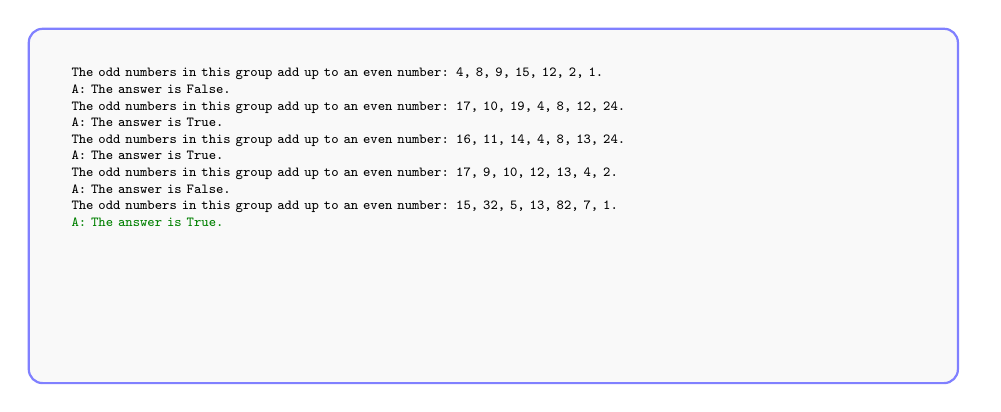
\begin{tikzpicture}
      % Outer rounded rectangle with blue border
      \node[draw=blue!50, thick, rounded corners=5pt, fill=gray!5, minimum width=11.8cm, minimum height=4.5cm, anchor=north west, inner sep=0pt] (fsbox) at (0,2.7) {};

      % Main multi-line code block in gray font, monospaced
      \node[anchor=north west, font=\ttfamily\tiny, text width=11.2cm, align=left, inner sep=2.5mm] at ([xshift=0.3cm, yshift=-0.26cm]fsbox.north west) {%
The odd numbers in this group add up to an even number: 4, 8, 9, 15, 12, 2, 1.\\
A: The answer is False.\\

The odd numbers in this group add up to an even number: 17, 10, 19, 4, 8, 12, 24.\\
A: The answer is True.\\

The odd numbers in this group add up to an even number: 16, 11, 14, 4, 8, 13, 24.\\
A: The answer is True.\\

The odd numbers in this group add up to an even number: 17, 9, 10, 12, 13, 4, 2.\\
A: The answer is False.\\

The odd numbers in this group add up to an even number: 15, 32, 5, 13, 82, 7, 1.\\
\textcolor{green!50!black}{A: The answer is True.}
      };
    \end{tikzpicture}
  \end{center}

\end{frame}
